\documentclass[../document.tex]{subfiles}
%\documentclass{beamer}
\usepackage{amssymb,amsmath,amsthm}
\usepackage{graphicx}
\usepackage{tikz}
%\usetheme{Singapore}
\usetheme{Boadilla}
\usecolortheme{rose}

\usetikzlibrary{tikzmark}
\usepackage{colortbl}
\usepackage{graphicx}
\usepackage{pdfpages}
\tikzstyle{every picture}+=[remember picture,baseline]
\tikzstyle{every node}+=[inner sep=0pt,anchor=base,
minimum width=1.5cm,align=center,text depth=.25ex,outer sep=1.5pt]
\tikzstyle{every path}+=[thick, rounded corners]
%\setframetemplate{frametitle}[default][center]

%%%%%%%%%%%%%%%%%%%% VERY IMPORTANT 
%very useful way to add notes to Beamer
%\setbeameroption{show notes on second screen=right}
\setbeamertemplate{note page} 
{ 
	\insertslideintonotes{0.65} 
	\rule{\textwidth}{0.1pt} 
	\color{blue} \small
	\insertnote 
}

\begin{document}
\begin{frame}[label=works]
	\frametitle{Brief history of Lamport's works}
	\begin{tikzpicture}[remember picture,overlay]
		\node [below= 1.9cm, left=0.8cm] at(current page.north east) { %for relative positioning, we use \node [left=1cm or right or below or above] 
			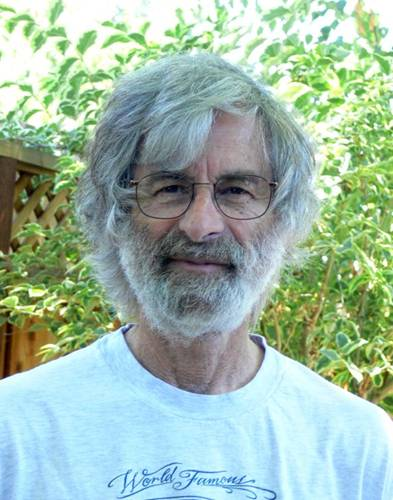
\includegraphics[width=0.24\textwidth]{lam.jpg}	
		};
	\end{tikzpicture}
	\begin{itemize}
		\item<1-> \textbf{Inventing \LaTeX: }\small a group of macros, which can make the life of \TeX users a lot easier!!
		\item<1-> \textbf{One way authentication} in Whitfield Diffie's "\textit{New directions in cryptography"} (1976)
	\end{itemize}
\end{frame}

%%%%%%%%%

\begin{frame}{brief description of \textbf{One-way Function}}
	\begin{itemize}
		\item<1-> A one way function \pmb{$f$} is a function that is \textbf{easy to compute } but whose \textbf{inverse is difficult to compute}: 
		\item<2-> or to say $f$ is one-way function iff (adapted from\footnotemark):
		\begin{enumerate}
			\item<3-> for all value $v$, finding data object $d$ s.t. $\phi(d)=v$ is \textbf{computationally infeasible.}
			\item<4-> $f$ is not \textbf{one-to-one} or proving it otherwise is \textbf{computationally infeasible.}\footnotemark 
		\end{enumerate}
	\end{itemize}
	\uncover<5->{ \centering 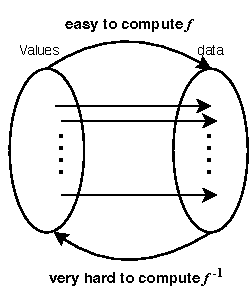
\includegraphics[width=0.3\textwidth]{../myfig1.pdf}}
	\footnotetext[1]{\footnotesize Lamport, "\textit{Constructing Digital Signatures from a One Way	Function}"}
	\footnotetext[2]{\footnotesize i.e. to say: $\forall$ data object $d' \ne d: \phi(d') \ne \phi(d)$}
\end{frame}

%%%%%%%%%

\begin{frame}{brief description of \textbf{One-way Authentication}}
	\begin{definition}[Digital signature]
		A digital signature created by \textbf{sender P} for \textbf{document m} is a data item $\sigma_p (m)$ that is when received together with \textbf{m}, one can determine (e.g. in a court of law) that \textbf{P} generated document \textbf{m}.\\
		\uncover<2->{Hence A tool for determining \textbf{validity} of something sent.\footnotemark}
	\end{definition}
	
	\footnotetext[1]{\footnotesize Lamport, L. (1979) "\textit{Constructing Digital Signatures from a One Way	Function}"}
\end{frame}

%%%%%%%%%

\begin{frame}{brief description of \textbf{One-way Authentication}}
	\begin{definition}[One way authentication]
		It must be \textbf{easy for anyone} to recognize the signature as \textbf{authentic} but \textbf{impossible} for anyone other than the signer to produce it!\footnotemark
	\end{definition}
	\footnotetext[1]{\footnotesize Diffie, W. (1976)"\textit{New Directions in Cryptography}"}
\end{frame}

%%%%%%%%%%%%

\begin{frame}{A practical Example of a \textbf{One-way function} in \textbf{one-way authentication} \\ \ \textbf{Login Problem}}
	\begin{itemize}
		\item<1-> User \textbf{A} enters Password \textbf{$PW$} and computer store it as \textbf{$f(PW)$} 
		\item<2-> where $f(PW)$ is a one-way function of \underline{10 million instructions}
		\item <3-> and its inverse has $10^{30}$ more instructions (or computations), which practically makes it \textbf{noninvertible}
		\item <4-> for example, finding square root of $x_0$ given in $f(x)=x^2$ is much harder than computing $x^2$ at $x_0$.
	\end{itemize}
\end{frame}

%%%%%%%%

\begin{frame}{brief description of \textbf{One-way Authentication} \textit{Cont'd}}
	\begin{itemize}
		\item <1-1>However, determining exactly what the one-way function should be is originally solved by \textbf{Lamport} \\ which further lead to the publication of the paper: "\textit{Constructing Digital Signatures from a One Way Function}"
		\item<2-> But how this solution relates to the ecosystem of \textbf{public keys} is \underline {out of the scope of the presentation} and discussed in the paper:\\ \textit{"New Directions in Cryptography"} by Whitfield Diffie (1976) 
	\end{itemize}
\end{frame}

%%%%%%%%%%%%%
\begin{frame}[label=works]
	\frametitle{Brief history of Lamport's works}
	\begin{itemize}
		\item<1-> \textbf{Inventing \LaTeX: }\small a group of macros, which can make the life of \TeX users a lot easier!!
		\item<1-> \textbf{One way authentication} in Whitfield Diffie's "\textit{New directions in cryptography"} (1976)
		\item <1-> \textbf{bakery algorithm} an algorithm to ensure mutual exclusion in concurrent processes
		\item <2->  that is to ensure a data structure is modified by at most one process at a time
		\\ and no process is reading a data structure while it is being written by other processes. 
		\item <3-> \textbf {Paxos algorithm}: an algorithm used in distributed systems for reaching consensus, used in distributed storage systems
	\end{itemize}
	\footnotetext[1]{Silberschatz, "Database System Concepts", Ch. 19, P. 965}
\end{frame}
%%%%%%%%%%%%%

\begin{frame}
	\frametitle{Brief history of Lamport's works \textit{cont'd}}
	\begin{itemize}
		\item <1-> Time, clocks and ordering of events in a distributed system:
		\begin{itemize}
			\item<2-> \footnotesize in a distributed system, sometimes it is \textbf{impossible} to say an event has happened before something else. 
			\item <3-7> \footnotesize hence, relation "\textit{happened before} is a partial ordering relation.
			\item <4-5> \textbf{Partial ordering? sounds familiar...}
			\alt<5> {\begin{definition} [Partial ordering]
					Partial ordering relation is an ordering relation in which not all members of the set need to be comparable!
			\end{definition}}{}
			\item <6-> \footnotesize He proposed in that paper a partial ordering of "happened before" and gave a \textbf{distributed algorithm} for \textbf{extending it to a total ordering of events}
			\newline \newline
			
			
		\end{itemize}
	\end{itemize}
	\uncover<7-> {\centering \large \textbf{But where is the "Byzantine generals" problem in the list?}}
	%\only{hi}<6>
\end{frame}
\end{document}